\documentclass[aspectratio=169]{beamer}

\usepackage[utf8]{inputenc}
\usepackage[T1]{fontenc}
\usepackage[portuguese]{babel}
\usepackage{graphicx}
\usepackage{booktabs}
\usepackage{array}

\usetheme{Singapore}

\title[PHVD-APS - Artefato e Experimentos]{Planejamento de Visitas Domiciliares na APS}
\subtitle{INF99003 - Projeto 2 - Grupo D}
\author{Fabio, Tobias e Vítor}
\date{Semana 3 - 01/10/2026}

\setbeamertemplate{navigation symbols}{}
\setbeamercovered{transparent}
\setbeamertemplate{footline}[frame number]

\definecolor{myblue}{RGB}{30,80,160}
\definecolor{myorange}{RGB}{210,100,20}

\begin{document}

\begin{frame}
  \titlepage
\end{frame}

\section{Artefato}
\begin{frame}{Artefato criado}
  \begin{columns}[T]
    \column{0.48\textwidth}
      \textbf{Monorepo em TypeScript}
      \begin{itemize}
        \item \textbf{Core}: planejamento, validação e otimização
        \item \textbf{Server}: API Fastify e banco SQLite
        \item \textbf{Web}: interface React com mapa Leaflet
      \end{itemize}
    \column{0.48\textwidth}
      \textbf{Fluxo principal}
      \begin{enumerate}
        \item Carregar ou criar um cenário
        \item Gerar o plano de visitas
        \item Visualizar e exportar rotas
        \item Registrar resultados e replanejar
      \end{enumerate}
  \end{columns}
  \vspace{0.6em}
  \centering
  \textcolor{myblue}{\textbf{O mesmo núcleo atende a interface e aos experimentos.}}
\end{frame}

\section{Métodos}
\begin{frame}{Três abordagens comparadas}
  \begin{columns}[T]
    \column{0.31\textwidth}
      \textbf{Urgência}
      \begin{itemize}
        \item Ordena por vencimento
        \item Insere na equipe viável
        \item \textcolor{myblue}{Foco: pendências}
      \end{itemize}
    \column{0.31\textwidth}
      \textbf{Vizinho mais próximo}
      \begin{itemize}
        \item Escolhe a visita mais próxima
        \item Constrói a rota geograficamente
        \item \textcolor{myblue}{Foco: deslocamento}
      \end{itemize}
    \column{0.31\textwidth}
      \textbf{Heurística 1.5-opt}
      \begin{itemize}
        \item Combina urgência e antecipação
        \item Usa custo incremental
        \item \textcolor{myblue}{Foco: equilíbrio}
      \end{itemize}
  \end{columns}
  \vspace{0.5em}

  \textcolor{myblue}{Mesmo cenário, calendário, capacidade e eventos para os três métodos.}
\end{frame}

\section{Núcleo}
\begin{frame}{Pipeline da nossa estratégia}
  \centering
  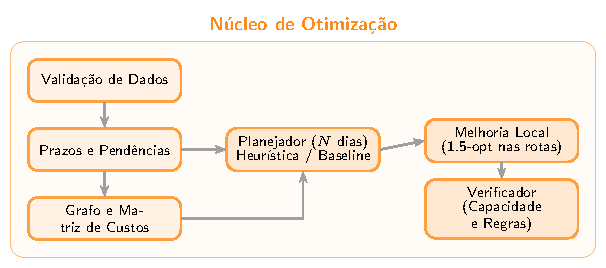
\includegraphics[width=1.0\textwidth,height=0.78\textheight,keepaspectratio]{figs/otimization_pipeline.pdf}
\end{frame}

\section{Resultados}
\begin{frame}{Resultados brutos}
  \centering
  \small
  \textbf{Benchmark estático: 33 registros} \hspace{1em} \textbf{Simulação dinâmica: 132 registros}
  \vspace{0.8em}

  \begin{tabular}{@{}lrrr@{}}
    \toprule
    \textbf{Método} & \textbf{Cobertura} & \textbf{Atraso (dias)} & \textbf{Distância (km)} \\
    \midrule
    Heurística 1.5-opt & 100,00\% & 116,91 & 90,59 \\
    Baseline de urgência & 99,09\% & 120,64 & 103,68 \\
    Baseline geográfico & 100,00\% & 114,36 & 62,61 \\
    \bottomrule
  \end{tabular}
\end{frame}

\begin{frame}{Leitura dos resultados}
  \begin{block}{Leitura principal}
    A heurística reduz o atraso em relação à urgência e mantém cobertura total. O baseline geográfico percorre menos quilômetros, mas não domina os demais critérios.
  \end{block}

  \vspace{0.6em}
  \begin{itemize}
    \item Sob falhas, cobertura e atraso pioram para todos os métodos.
    \item A heurística oferece um compromisso entre cobertura e atraso.
    \item Pareto, sensibilidade e escala ainda serão aprofundados.
  \end{itemize}
\end{frame}

\begin{frame}{}
  \centering
  \vspace{1cm}
  {\Huge Obrigado!}\\[1em]
  {\large Dúvidas e discussão}
\end{frame}

\end{document}
\endinput